La réalisation de ce travail de Bachelor a nécessité une gestion précise du temps et des ressources. Pour assurer une progression régulière et structurée du projet, une méthodologie de travail spécifique a été mise en place. Cette méthodologie a été centrée autour de quatre piliers principaux : la planification, le suivi du temps, la gestion du cahier de bord et la documentation. Ces piliers ont permis de maintenir une approche disciplinée et organisée tout au long du développement, garantissant ainsi une livraison en temps et en heure tout en assurant la qualité du produit final.

\section{Planification et Organisation}

La planification et l'organisation du travail étaient une composante essentielle de la méthode de travail utilisée tout au long du développement du système. Pour ce faire, une approche basée sur l'utilisation d'un tableau blanc a été adoptée. Cette méthode, bien que simple, s'est avérée extrêmement efficace pour gérer le workflow du projet.

Le tableau blanc a été utilisé pour décomposer le projet en une série de tâches plus petites. Ces tâches ont été organisées en sprints, qui sont des périodes de travail dédiées à l'accomplissement d'un ensemble spécifique de tâches. En règle générale, en début de semaine, une session de planification était effectuée pour définir et prioriser les tâches à accomplir pendant le sprint.

Cette méthode a offert un certain nombre d'avantages. Tout d'abord, elle a permis de maintenir une vue d'ensemble claire du projet, facilitant ainsi le suivi de son avancement. Deuxièmement, elle a offert la flexibilité nécessaire pour ajuster la planification en fonction de l'évolution du projet. Enfin, en ayant le tableau constamment visible, il était possible de rester concentré sur les objectifs actuels et à venir.

\begin{figure}[H]
    \centering
    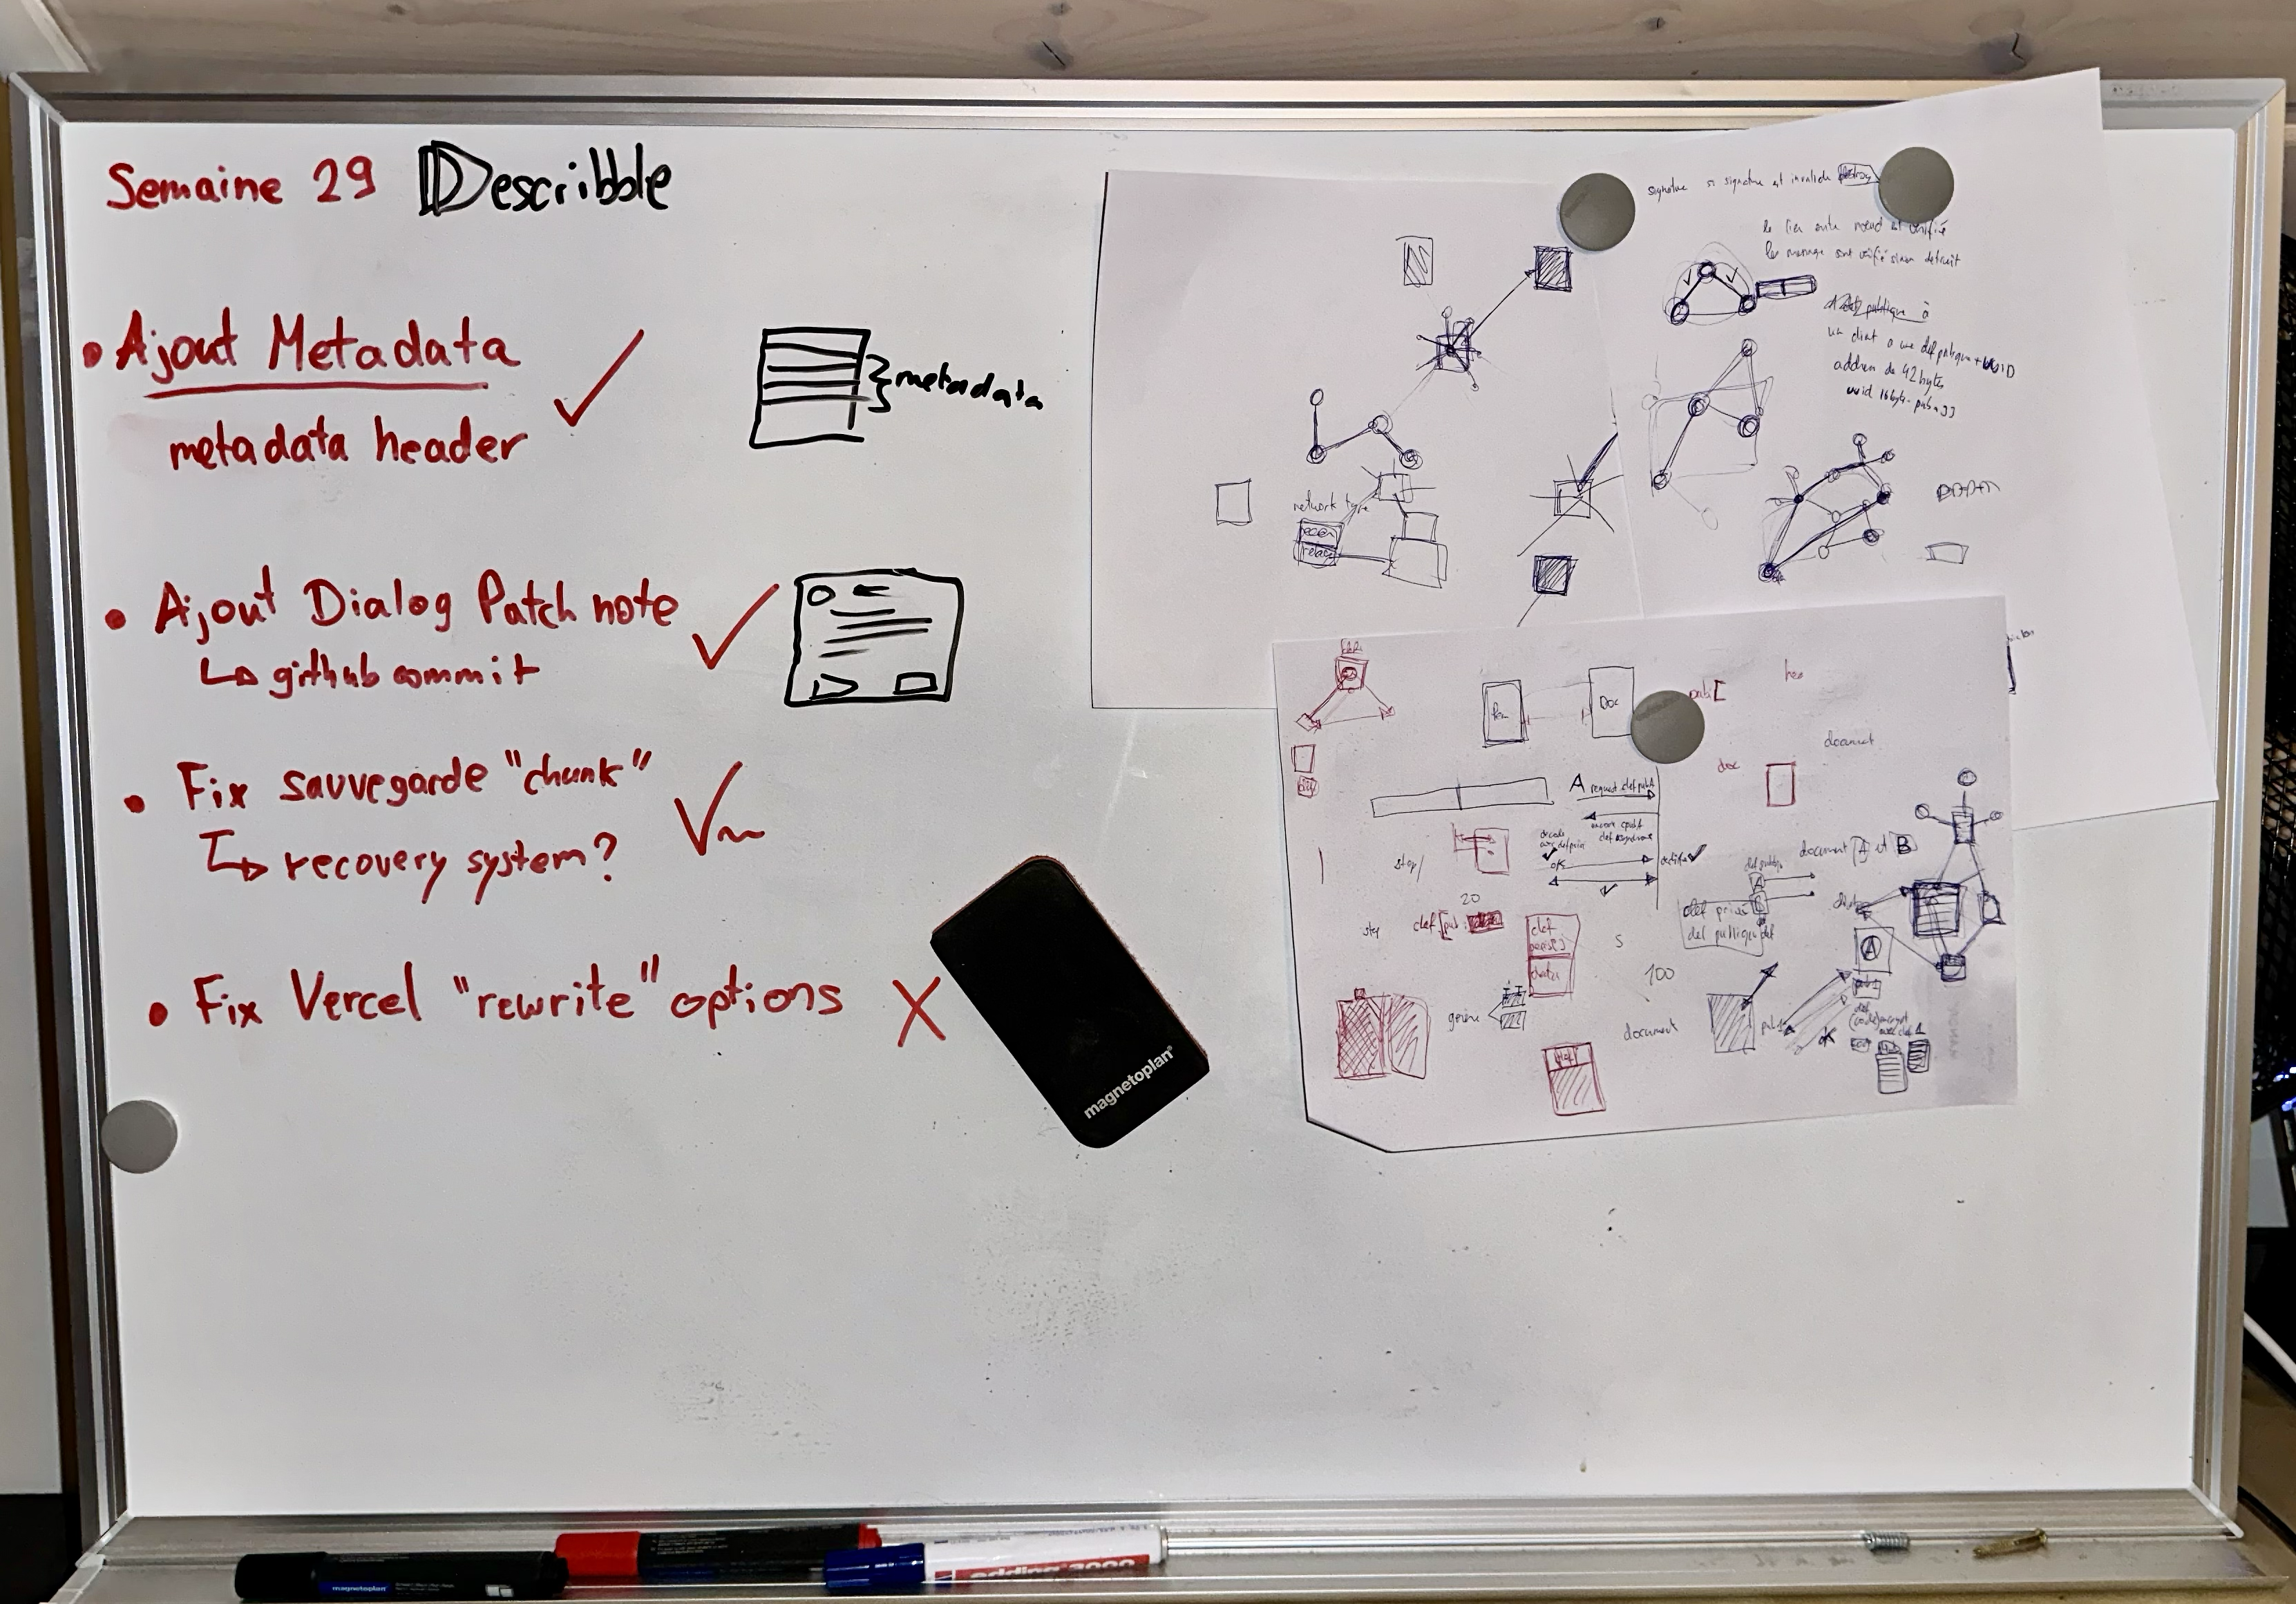
\includegraphics[width=0.9\textwidth]{assets/figures/planning.png}
    \caption{Exemple de planification sur un tableau blanc}
\end{figure}

Il convient de noter que cette méthode de planification a bien fonctionné compte tenu du fait que le développement a été effectué seul. Si le projet avait été réalisé par une équipe plus grande, il aurait été nécessaire d'utiliser des outils de gestion de projet plus formels, tels que Trello ou Jira. Cependant, dans le contexte de ce projet, cette méthode s'est avérée adaptée, en particulier compte tenu du fait que le travail était principalement effectué à domicile, avec le tableau blanc constamment sous les yeux.

\section{Documentation}

La documentation a été un autre aspect essentiel de la méthodologie de travail. Chaque portion de code produite a été soigneusement documentée. Cela avait pour but de faciliter la compréhension du projet pour quiconque souhaitant le comprendre ou y contribuer à l'avenir.

En plus de documenter le code, le projet a été publié sous forme de paquets sur le gestionnaire de paquets \gls{Node.js} (\gls{npm}). Ces paquets ont été soigneusement documentés pour permettre à d'autres développeurs de comprendre leur fonctionnement et de les utiliser dans leurs propres projets. La documentation des paquets \gls{npm} est particulièrement importante, car elle fournit aux développeurs des informations cruciales sur la manière d'installer et d'utiliser les paquets.

Le projet a été hébergé sur GitHub, accessible à l'adresse \url{https://github.com/maxscharwath/describble}. Le dépôt a été maintenu dans un état propre et bien organisé. Cela a permis de faciliter la navigation à travers le projet et d'améliorer sa maintenabilité.

\begin{figure}[H]
    \centering
    \includegraphics[width=0.9\textwidth]{assets/figures/npm-package.png}
    \caption{Exemple de paquet publié sur \gls{npm} avec une documentation détaillée. Le paquet peut être trouvé à l'adresse suivante: \url{https://www.npmjs.com/package/@describble/ddnet.}}
\end{figure}

\section{Gestion du cahier de bord}

La gestion du cahier de bord a été une composante essentielle de la méthodologie de travail. Ce processus a été principalement réalisé en documentant chaque commit. Ces documents ont non seulement servi de cahier de bord, mais ont également été utilisés pour générer automatiquement des notes de version.

Ces notes de version, affichées dans une fenêtre de dialogue accessible par l'interface utilisateur de l'application, fournissent un aperçu rapide et facile des modifications apportées à chaque version. Pour afficher cette fenêtre, l'utilisateur doit simplement cliquer sur le numéro de version situé dans le pied de page de l'interface. Une fenêtre s'ouvre alors, révélant la liste des dernières notes de version. Chaque entrée liste le numéro de version, la date de publication, et un résumé concis des modifications apportées dans cette version.

\begin{figure}[H]
    \centering
    \includegraphics[width=0.9\textwidth]{assets/figures/patch_notes.png}
    \caption{Dialogue affichant les notes de version dans l'application}
\end{figure}

Cette fonctionnalité offre une transparence supplémentaire sur le processus de développement et permet aux utilisateurs de rester informés des dernières mises à jour et améliorations. En outre, elle encourage l'interaction continue entre les utilisateurs et les développeurs, favorisant ainsi l'évolution constante de l'application.